% !TEX root = ../bachlor-arbeit.tex
\begin{figure}[H]
    \centering
    \includegraphics[width=.9\linewidth]{al_algo_new}
    \caption[]{The algorithm tries to find to a given transmission spectrum $I$ the design parameters $\mc D$ of a two layer meta surface stack which can reproduce this target. The input spectrum is passed to a convolutional neural network which outputs its guess for the stack and layer parameters. The Database module looks at the two sets of layer parameters and interpolates between stored $S$-matrices to give an estimate for the two $S$-matrices describing the layers. The SASA algorithm calculates the resulting current transmission spectrum and passes it to the optimizer. This last module compares it to the target spectrum and adjusts the continuous parameters to minimize the difference between the two spectra. Find the details to all parts of the algorithm in the sections below.}
    \label{fig:al:algo}
\end{figure}
\vspace{0.2cm}

\begin{tabular}{ll}
    \vspace{0.64cm}
    \hyperref[sec:NN]{NN}: &
    \begin{tabular}[t]{@{}l@{}}
        convolutional neural network trained to map spectra to stack and \\ layer parameters
    \end{tabular}\\
    %
    \vspace{0.64cm}
    \hyperref[sec:DB]{DB}: &
    database of pre-simulated single layers\\
    %
    \vspace{0.64cm}
    \hyperref[sec:SASA]{SASA}: &
    algorithm calculating $\hat{S}_\s{stack} = \hat{S}_\s{stack}(\hat{S}_1, \, \hat{S}_2, \, \varphi, \, h)$\\
    %
    \vspace{0.64cm}
    \hyperref[sec:opt]{Opt}: &
    \begin{tabular}[t]{@{}l@{}}
        optimizer changing the continuous parameters to minimize the difference \\
        between the current and target spectrum
    \end{tabular}\\
    %
    \vspace{0.64cm}
    $\hat{S}_1, \, \hat{S}_2$ &
    S-matrices of the top and bottom layer\\
    %
    \vspace{0.64cm}
    $\mc L_1 , \, \mc L_2$ &
    \begin{tabular}[t]{@{}l@{}}
        two sets of layer parameters where
        $\mc L = (w, \, l, \, t, \, \Lambda, \, m, \, g)$ \\
        $w$...width, $l$...length, $t$...thickness, $\Lambda$...Period,
        $m$...material, $g$...geometry
    \end{tabular}\\
    %
    \vspace{0.64cm}
    $\mc S$ &
    \begin{tabular}[t]{@{}l@{}}
        stack parameters $\mc S = (d, \varphi)$ where \\
        $d$...distance between layers, $\varphi$...rotation angle\\
    \end{tabular}\\
    %
    \vspace{0.64cm}
    optimization loop & this loop is repeated until the target accuracy is reached\\
    %
    \vspace{0.64cm}
    $I$ & input transmission spectrum\\
    %
    \vspace{0.64cm}
    $\mc D$ & output design parameters\\
\end{tabular}
